\documentclass[12pt]{article}

% Load packages
\usepackage{url}
\usepackage{ifthen}
\usepackage{multicol}
\usepackage[utf8]{inputenc}
\usepackage{amsmath}
\usepackage{amssymb}
\usepackage{graphicx}
\usepackage[margin=0.1pt,font=footnotesize,labelfont=bf]{caption}
\usepackage{setspace}
\usepackage{colortbl}
\usepackage[square,sort,comma,numbers,sort&compress]{natbib}
\usepackage{fullpage}
\usepackage{textcomp}
\usepackage{lineno}
\usepackage{booktabs}
\usepackage{longtable}

\urlstyle{rm}

\bibliographystyle{plos2009}

\makeatletter
\renewcommand\subsection{\@startsection
	{subsection}{2}{0mm}
	{-0.05in}
	{-0.5\baselineskip}
	{\normalfont\normalsize\bfseries}}
\renewcommand\subsubsection{\@startsection
	{subsubsection}{2}{0mm}
	{-0.05in}
	{-0.5\baselineskip}
	{\normalfont\normalsize\itshape}}
\renewcommand\section{\@startsection
	{subsection}{2}{0mm}
	{-0.2in}
	{0.05\baselineskip}
	{\normalfont\large\bfseries}}
\renewcommand\paragraph{\@startsection
	{paragraph}{2}{0mm}
	{-0.05in}
	{-0.5\baselineskip}
	{\normalfont\normalsize\itshape}}
\makeatother

\linenumbers

% Single space'd bib
\setlength\bibsep{0pt}

\renewcommand{\rmdefault}{phv}\renewcommand{\sfdefault}{phv}
\newcommand{\norm}[1]{\left\lVert#1\right\rVert}

% Change the number format in the ref list
\renewcommand{\bibnumfmt}[1]{#1.}

% Change Figure to Fig.
\renewcommand{\figurename}{Fig.}

% Begin document
\begin{document}
\doublespacing
\begin{titlepage}
{\par\centering\textbf{\Large {Mechanistic Resource Competition Modeling of a Cell-Free Gluconate Biosensor}}}
\vspace{0.05in}
{\par \centering \large{Abhinav Adhikari, Abhishek Murti, Anirudh M. Narayanan, Ha Eun Lim, and Jeffrey D. Varner\,$^{*}$}}
\vspace{0.10in}
{\par \centering {Robert Frederick Smith School of Chemical and Biomolecular Engineering}}
{\par \centering {College of Engineering, Cornell University, Ithaca, NY 14853}}
\vspace{0.1in}
{\par \centering \textbf{Running Title:}~Mechanistic Resource Model for Cell-Free Biosensors}
\vspace{0.1in}
{\par \centering $^{*}$Corresponding author:}
{\par \centering Jeffrey D. Varner,}
{\par \centering Professor, School of Chemical and Biomolecular Engineering,}
{\par \centering 244 Olin Hall, Cornell University, Ithaca NY, 14853}
{\par \centering Email: jdv27@cornell.edu}
{\par \centering Phone: (607) 255 - 4258}
{\par \centering Fax: (607) 255 - 9166}
\end{titlepage}
\date{}
\thispagestyle{empty}
\pagebreak

\section*{Abstract}
Cell-free synthetic biology systems offer a promising platform for rapid prototyping of biosensor circuits because they eliminate the confounding effects of cellular growth and membrane transport. However, the finite transcriptional and translational resources in cell-free reactions impose time-dependent capacity constraints that are difficult to capture with empirical decay functions. In this study, we developed and validated a mechanistic resource competition model for a D-gluconate biosensor circuit operating in the reconstituted cell-free system PURExpress. The circuit employed the transcription factor GntR to repress expression of the fluorescent reporter Venus, with D-gluconate relieving repression in a dose-dependent manner. We formulated a two-layer resource model in which the first layer described the allocation of RNA polymerase and ribosome between competing genes using Michaelis-Menten-like expressions, and the second layer captured the irreversible depletion of consumable resources (nucleotides, energy cofactors, and amino acids) through ordinary differential equations driven by cumulative transcription and translation flux. This mechanistic formulation replaced the ad hoc logistic and exponential decay functions commonly used in cell-free models while providing a physical interpretation of resource exhaustion. Model parameters were estimated using a multi-objective and single-objective cycling strategy implemented in ParetoEnsembles.jl, yielding an ensemble of $N = 78$ parameter sets that captured the transcription and translation kinetics of the circuit. The model predicted that 76\% of transcriptional resources and 2\% of translational resources were consumed by 12 hours, consistent with the observed saturation of mRNA and protein trajectories. Without re-estimation of parameters, the model accurately predicted the dose-response relationship of Venus protein as a function of D-gluconate concentration over four orders of magnitude, yielding a dissociation constant of $K_{\text{gluconate}} = 0.13 \pm 0.01$ mM and a Hill coefficient of $n_{\text{gluconate}} = 2.36 \pm 0.34$. Taken together, this study demonstrated that a mechanistic resource competition framework improved the predictive capability and interpretability of cell-free biosensor models and provided quantitative design rules for the allocation of transcriptional and translational capacity in synthetic gene circuits.

\vspace{0.1in}
{\noindent \textbf{Keywords:}~cell-free biosensors, mathematical modeling, synthetic biology, resource competition, parameter estimation, transcription-translation dynamics}

\clearpage

\section*{Introduction}
Synthetic biology seeks to program biological systems to perform user-specified functions. Traditionally, synthetic biology involved engineering the functionality of living cells using genetic tools; however, recent applications have increasingly focused on cell-free platforms, which offer several advantages over their in vivo counterparts \cite{Swartz2018,silverman2020cell,Bundy_2018,CFPS-Review-2020,garenne2021cell,moore2017cell,hunt2025cellfree}. The absence of cellular growth and maintenance requirements, together with the removal of the cell wall barrier, facilitates the interrogation and manipulation of reaction conditions and directs the allocation of carbon and energy resources toward a product of interest. Furthermore, cell-free platforms enable the use of linear DNA fragments instead of plasmids, which significantly reduces the time required for design-build-test cycles. Fundamentally, a cell-free system includes only the components required for transcription and translation (TXTL) processes, such as RNA polymerase (RNAP), ribosomes, transcription and translation elongation factors, energy compounds, salts, amino acids, and ribonucleotides. There are two classes of cell-free systems: reconstituted and extract-based. Extract-based systems are prepared by lysing whole cells and separating the unwanted debris, while reconstituted systems are well-defined and prepared using only the factors essential for protein synthesis, including purified enzymes, tRNAs, ribosomes, elongation factors, amino acids, and energy molecules. The well-defined composition of reconstituted systems makes them an attractive platform for studying biomolecular interactions and for quantitative modeling without the confounding effects of unknown components present in extract-based systems \cite{Vilkhovoy:2018aa,Horvath2020,karzbrun2011coarse}.

One promising application area for cell-free systems is biosensing. Traditionally, biosensors based on live cells have faced a significant challenge: transport limitations caused by the cell membrane. Cell-free biosensors overcome this barrier by removing the constraint of the cell membrane and allowing direct access to the transcription and translation machinery, which leads to increased sensitivity and faster response times. Transcription-factor-based biosensors, which utilize a transcription factor that is allosterically modified upon binding to a small molecule to control the expression of a reporter gene, are predominantly used to detect small molecules and ions. Such sensing systems have recently been used to detect water contaminants, biomarkers, and antibiotics \cite{soltani2018reengineering,grawe2019paper,voyvodic2020cell,jung2020cell,pardee2014based,wen2017cell,li2025cellfree,mcsweeney2025modular}. Because cell-free systems can be freeze-dried and later reconstituted with water, they can be deployed for on-demand, point-of-care applications \cite{jung2020cell}. Moreover, the detection range of existing transcription factors can be expanded through metabolic engineering; for example, Voyvodic and coworkers used the transcription factor BenR to detect benzoic acid and then employed metabolic enzymes to convert hippuric acid and cocaine into benzoic acid, thereby broadening the spectrum of detectable molecules \cite{voyvodic2019plug}.

Despite the experimental progress in cell-free biosensors, quantitative mathematical models that capture the full dynamics of these systems remain underdeveloped. A central challenge is the finite and non-renewable nature of transcriptional and translational resources in cell-free reactions. As nucleotides, amino acids, and energy cofactors are consumed, the rates of mRNA and protein production decline in ways that are difficult to predict from first principles. Several groups have developed resource-aware models for gene expression systems. Gyorgy and Murray developed a framework for resource competition in synthetic genetic circuits where shared cellular machinery couples otherwise independent modules \cite{gyorgy2016resource}. Weisse et al. proposed a whole-cell model in which host and circuit compete for a shared ribosome pool \cite{weisse2015mechanistic}. In the cell-free context, Stogbauer et al. characterized the time-dependent loss of translational activity in extract-based systems due to ribosome inactivation \cite{stogbauer2012experiment}, Karzbrun et al. developed a coarse-grained model of TX/TL dynamics \cite{karzbrun2011coarse}, and Vilkhovoy et al. used constraint-based modeling to evaluate the performance limits of \emph{E.~coli} cell-free protein synthesis \cite{Vilkhovoy:2018aa}. More recently, Piorino et al. experimentally characterized plasmid crosstalk in cell-free expression systems \cite{piorino2023plasmid}, and Han et al. developed a mathematical model that explicitly captured resource competition between co-expressed genes \cite{han2025mathematical}. Yurchenko et al. reviewed both mechanism-based and data-driven modeling approaches for cell-free synthetic biology \cite{yurchenko2024mechanism}, while Ganesh and Maerkl explored the performance limits of the PURE reconstituted system \cite{ganesh2024towards}. However, despite this progress, existing cell-free models have generally treated resource depletion using empirical decay functions (e.g., logistic or exponential functions of time) that lack a mechanistic basis and do not couple resource consumption to the actual biosynthetic load on the system.

In this study, we developed a mechanistic two-layer resource competition model for a D-gluconate biosensor circuit operating in the reconstituted cell-free system PURExpress. D-gluconate was chosen as the target analyte because its cognate transcription factor, GntR, is well-characterized in \textit{Bacillus subtilis}, \textit{Escherichia coli}, and \textit{Pseudomonas aeruginosa} \cite{Miwa1988,Fujita1989,Peekhaus1998,Yoshida1995,daddaoua2017identification}, and because gluconate detection is relevant to food safety and industrial fermentation monitoring, where D-gluconate serves as an indicator of microbial activity and product quality \cite{ramachandran2006gluconic}. The first layer of the resource model described the allocation of RNA polymerase and ribosome between competing transcription units using Michaelis-Menten-like saturation expressions, while the second layer captured the irreversible depletion of consumable resources through differential equations driven by the cumulative transcription and translation flux. This formulation replaced the previous empirical decay functions with a physically interpretable framework and simultaneously reduced the number of estimated parameters. We estimated model parameters using a multi-objective optimization approach implemented in ParetoEnsembles.jl, which cycled between multi-objective Pareto front exploration and single-objective refinement. The resulting model accurately captured the time-resolved mRNA and protein dynamics under training conditions and, without re-estimation of parameters, predicted the dose-response relationship of Venus protein as a function of D-gluconate concentration over four orders of magnitude.

\clearpage
\section*{Materials and Methods}

\subsection*{Construction of the gluconate-responsive transcription units.}
Design of the transcription unit was adapted from the P70 series developed by Noireaux and coworkers \cite{shin2010efficient}. A 16 bp \textit{E.~coli} GntR operator (ATGTTACCCGTATCAT) was added between the $-35$ and $-10$ region of the P70 promoter. The $-10$ binding site of the RpoD holoenzyme was altered as a result from \textit{GATAAT} in the original promoter to \textit{TATCAT} in our modified P70 promoter (mP70). The gene sequence of the reporter protein (Venus) was added downstream of this modified promoter. The 5-prime untranslated region and the T500 terminator were unchanged from ref \cite{shin2010efficient}. The second transcription unit had the GntR repressor gene downstream of the original (P70) promoter (without the GntR operator). The full constructs were ordered as linear DNA fragments, with 150--200 bp flanker sequences on both ends, from Twist Bioscience. The sequences of the GntR operator and the repressor were obtained from the literature \cite{Peekhaus1998,izu1997gene}.

\subsection*{Cell-free protein synthesis reactions.}
The cell-free protein synthesis (CFPS) reactions were carried out using the PURExpress In Vitro Protein Synthesis Kit (New England Biolabs Inc) in 384-well plates (Thermofisher NUNC, flat-bottom) in a Varioskan Lux plate reader at 37$^{\circ}$C. The working volume of all reactions was 25 $\mu$L, composed of the PURE solutions A (10 $\mu$L) and B (7.5 $\mu$L), RNase inhibitor, Murine (0.5 $\mu$L), NEB \textit{E.~coli} RNA Polymerase holoenzyme (2 $\mu$L), and the linear DNA: Venus (7 nM), GntR (10 nM). For the control reactions without GntR, an equal volume of nuclease-free water was used in its stead. For the de-repression reactions, D-gluconate was added while maintaining the same total volume. The \textit{E.~coli} RNA Polymerase, Holoenzyme is the core enzyme saturated with sigma factor 70 and initiates RNA synthesis from sigma 70 specific promoters. The gene constructs were ordered as linear DNA fragments, with 150--200 bp flanker sequences on both ends, from Twist Bioscience. Prior to the cell-free protein synthesis reactions, the DNA fragments were PCR amplified using Q5\textsuperscript{\textregistered} Hot Start High-Fidelity 2X Master Mix (New England Biolabs Inc) following manufacturer instructions and the PCR reactions were purified using PureLink\texttrademark~PCR Purification Kit (Invitrogen).

\subsection*{mRNA quantification.}
Following each CFPS run, the total RNA was extracted from 5 $\mu$L of the reaction mixture using PureLink RNA Mini Kit (Thermo Fisher Scientific) and stored immediately at $-80^{\circ}$C. The quantitative RT-PCR reactions were done using Applied Biosystems\texttrademark~TaqMan\texttrademark~RNA-to-CT\texttrademark~1-Step Kit. An mRNA standard curve was used to determine absolute mRNA concentrations for each of the samples. The mRNA standards were prepared as follows: separate CFPS reactions for 5 nM of plasmids (Venus and GntR) were carried out for 2 hours. Total RNA was extracted using the full reaction volume. This was followed by the removal of 16S and 23S rRNA using the MICROBExpress\texttrademark~Bacterial mRNA Enrichment Kit (Life Technologies Corporation). Lastly, the MEGAclear\texttrademark~Kit (Life Technologies Corporation) was used to further purify the mRNA. The mRNA concentrations were determined using the Qubit\texttrademark~RNA assay kit (ThermoFisher Scientific).

\subsection*{Protein quantification.}
Venus fluorescence was measured using the Varioskan Lux plate reader at 513 nm (excitation) and 531 nm (emission). The fluorescence was measured with 25 $\mu$L for each of the mixtures. For all measurements, at least three biological replicates were performed. A protein standard curve was used to determine the absolute protein concentrations for each of the samples. The standard curve was prepared by using Venus standards of known concentration. To prepare the standards, histidine-tagged Venus was expressed using CFPS and purified using a Ni spin column (New England Biolabs). The concentration was measured using SDS-PAGE on Mini-PROTEAN Tetra Cell (Bio-Rad Laboratories) using Any kD\texttrademark~Mini-PROTEAN\textsuperscript{\textregistered} TGX Stain-Free\texttrademark~Protein Gels (Bio-Rad Laboratories). This was followed by staining the gel with Bio-Safe\texttrademark~Coomassie Stain (Bio-Rad Laboratories). The stained gel was visualized using the ChemiDoc MP and then the concentrations were measured using Image Lab software.

\subsection*{Formulation and solution of model equations.}
The model formulation built upon the effective biophysical modeling framework of Adhikari et al. \cite{adhikari2020effective}, with significant modifications to the resource limitation framework. The concentration of mRNA $m_j$ and protein $p_j$ for each gene $j$ were described using the balance equations:
\begin{eqnarray}
\label{eq:mrna_balance}
\dot{m}_j &=& r_{X,j}\,\bar{u}_j\,\epsilon_X - \theta_{m,j}\,m_j \\
\label{eq:prot_balance}
\dot{p}_j &=& r_{L,j}\,\bar{w}_j\,\epsilon_L - \theta_{p,j}\,p_j
\end{eqnarray}
where $r_{X,j}\bar{u}_j$ and $r_{L,j}\bar{w}_j$ denote the transcription and translation rates, respectively (units: concentration/time), and $\theta_{m,j}$ and $\theta_{p,j}$ denote the respective degradation rate constants (units: 1/time). The $\bar{u}_j(\dots) \in [0,1]$ and $\bar{w}_j(\dots) \in [0,1]$ terms describe the control input governing the transcription of gene $j$ and the translation of mRNA $j$, respectively. The $\epsilon_X(\dots) \in [0,1]$ and $\epsilon_L(\dots) \in [0,1]$ terms describe the availability of consumable transcriptional and translational resources, respectively, and are governed by differential equations described below.

\subsubsection*{Transcription and translation kinetics.}
The rate of transcription was modeled as the product of a kinetic limit $r_{X,j}$, a control term $\bar{u}_j(\dots) \in [0,1]$, and the consumable resource term $\epsilon_X(\dots) \in [0,1]$. The kinetic limit of transcription was derived from a four-step elementary reaction mechanism (RNAP binding, closed-to-open complex isomerization, abortive initiation, and productive elongation), as described previously \cite{adhikari2020effective} and detailed in the Supplementary Material (Section S1):
\begin{equation}
r_{X,j} = V_{X,j}^{\max}\left(\frac{\mathcal{G}_j}{\tau_{X,j}K_{X,j} + (\tau_{X,j}+1)\mathcal{G}_j}\right)
\end{equation}
where the initiation time constant $\tau_{X,j}$ and saturation constant $K_{X,j}$ were experimentally measured by McClure \cite{mcclure_1980}. The maximum transcription rate $V_{X,j}^{\max}$ was formulated as:
\begin{equation}
V_{X,j}^{\max} = R_{X,\text{free}}\left(\frac{\dot{v}_X}{l_{G,j}}\right)
\end{equation}
where $R_{X,\text{free}}$ denotes the free RNA polymerase concentration, $\dot{v}_X$ denotes the RNA polymerase elongation rate (nt/h), and $l_{G,j}$ denotes the length of gene $j$ in nucleotides. By analogy, the kinetic limit of translation was formulated as:
\begin{equation}
r_{L,j} = V_{L,j}^{\max}\left(\frac{m_j}{\tau_{L,j}K_{L,j} + (\tau_{L,j}+1)m_j}\right)
\end{equation}
where $m_j$ denotes the mRNA concentration and $V_{L,j}^{\max}$ denotes the maximum translation rate:
\begin{equation}
V_{L,j}^{\max} = K_P\,R_{L,\text{free}}\left(\frac{\dot{v}_L}{l_{P,j}}\right)
\end{equation}
where $R_{L,\text{free}}$ denotes the free ribosome concentration, $\dot{v}_L$ denotes the translation elongation rate (aa/s), $l_{P,j}$ denotes the length of protein $j$ in amino acids, and $K_P$ is a polysome amplification constant.

\subsubsection*{Transcription and translation control functions.}
The formulation of the control function $\bar{u}(\dots)$ was similar to the previous study of Adhikari et al. \cite{adhikari2020effective} and the earlier work of Moon et al. \cite{Moon:2012aa}, with pseudo-energy bounds informed by the analysis of Bintu et al. \cite{bintu2005transcriptional}. A detailed derivation of the partition function formalism and its application to each promoter in the gluconate sensor circuit is provided in the Supplementary Material (Section S3). Suppose the promoter $P$ can exist in one of $s = 1, 2, \dots, \mathcal{S}$ possible discrete independent microstates, where each microstate $s$ has some pseudo energy $\epsilon_s$. Some microstates will lead to transcription, while others will not. For each microstate $s$, let us assign a pseudo energy $\epsilon_s$, where $\epsilon_1 = 0$; we assumed the base state of a promoter $P$, i.e., the state in which nothing is bound to the promoter-DNA, has zero pseudo energy. Further, suppose the probability that promoter $P$ is in microstate $s$ follows a Boltzmann distribution:
\begin{equation}
p_i = \frac{1}{Z} \times f_i \exp\left(-\beta\epsilon_i\right) \qquad i = 1, 2, \dots, \mathcal{S}
\end{equation}
The quantity $p_i$ denotes the probability that promoter $P$ is in microstate $i$, $f_i$ denotes a state-specific factor $f_i \in [0,1]$ (typically a Hill-type expression describing the fraction of bound effector), $\beta$ denotes the thermodynamic beta, and $Z$ denotes a normalization factor. Using the summation law of discrete probability, $\sum_s p_s = 1$, the partition function is:
\begin{equation}
Z = \sum_{s=1}^{\mathcal{S}} f_s \exp\left(-\beta\epsilon_s\right)
\end{equation}
The control function $\bar{u}(\dots)$ was then computed as the probability that the promoter is in a transcription-competent microstate, given by the sum of probabilities over the subset $\mathcal{A} \subseteq \Omega$ in which transcription occurs:
\begin{equation}
\bar{u} = \sum_{s \in \mathcal{A}} p_s
\end{equation}
The translation control term $\bar{w}(\dots)$ was set to 1 due to the absence of a translational regulatory network in the current system.

\subsubsection*{Mechanistic resource competition model.}
A key contribution of this study was the replacement of ad hoc resource depletion functions (e.g., logistic or exponential decay in time) with a mechanistic two-layer resource competition framework. The first layer described the allocation of transcriptional and translational machinery between competing genes. The free RNA polymerase and ribosome concentrations were computed algebraically from the total concentrations $R_{X,T}$ and $R_{L,T}$ by accounting for the fraction of each machinery sequestered by active genes:
\begin{eqnarray}
\label{eq:RNAP_free}
R_{X,\text{free}} &=& \frac{R_{X,T}}{1 + \displaystyle\sum_j f_{X,j}} \\
\label{eq:Ribo_free}
R_{L,\text{free}} &=& \frac{R_{L,T}}{1 + \displaystyle\sum_j f_{L,j}}
\end{eqnarray}
where the sequestration fractions $f_{X,j}$ and $f_{L,j}$ were given by Michaelis-Menten-like expressions:
\begin{eqnarray}
f_{X,j} &=& \frac{\mathcal{G}_j}{\tau_{X,j}K_X + (1 + \tau_{X,j})\mathcal{G}_j} \\
f_{L,j} &=& \frac{m_j}{\tau_{L,j}K_L + (1 + \tau_{L,j})m_j}
\end{eqnarray}
These expressions arose naturally from the same initiation-elongation kinetics used to derive the transcription and translation rate laws (Supplementary Material, Section S2) and ensured that the allocation of machinery shifted dynamically as gene dosages and mRNA concentrations changed over time.

The second layer described the irreversible depletion of consumable resources (nucleotides, energy cofactors, amino acids, and related metabolites) that were not regenerated in the cell-free reaction. Two state variables, $\epsilon_X \in [0,1]$ and $\epsilon_L \in [0,1]$, represented the fractional availability of transcriptional and translational consumable resources, respectively. Their dynamics were governed by:
\begin{eqnarray}
\label{eq:epsX}
\frac{d\epsilon_X}{dt} &=& -\alpha_X \left(\sum_j l_{G,j}\,r_{X,j}\,\bar{u}_j\right)\epsilon_X \\
\label{eq:epsL}
\frac{d\epsilon_L}{dt} &=& -\alpha_L \left(\sum_j l_{P,j}\,r_{L,j}\right)\epsilon_L
\end{eqnarray}
with initial conditions $\epsilon_X(0) = 1$ and $\epsilon_L(0) = 1$. Here, $\alpha_X$ and $\alpha_L$ are consumption rate constants (units: inverse flux), $l_{G,j}$ is the gene length in nucleotides, and $l_{P,j}$ is the protein length in amino acids. The depletion rates were proportional to the total transcription and translation flux weighted by the respective sequence lengths, reflecting the stoichiometric requirement that longer genes consume more nucleotides per transcript and longer proteins consume more amino acids per polypeptide. This formulation ensured that resource depletion was driven by the actual biosynthetic activity in the system rather than by a predetermined time course, providing a mechanistic link between gene expression load and resource exhaustion.

\subsection*{Estimation of model parameters.}
Model parameter values were either taken from published studies, governed by experimental conditions, or estimated in this study. Unknown model parameters $\kappa$ were estimated by minimizing the squared difference between model simulations and experimental measurements. The minimization problem was formulated as a multi-objective optimization problem with six objectives:
\begin{equation}
\min_{\kappa}\;\mathcal{O}_k = \sum_{i \in \mathcal{E}_k}\left(\hat{\mathcal{M}}_{ik} - \hat{x}_{ik}(\kappa)\right)^2 \qquad k = 1, \dots, 6
\end{equation}
subject to:
\begin{eqnarray}
\label{eq:model-eqn}
\dot{x} &=& f(x, \kappa) \\
\label{eq:eqn-bounds}
\mathcal{L} \leq &\kappa& \leq \mathcal{U} \\
\label{eq:eqn-initial-condition}
x(t_0) &=& x_0
\end{eqnarray}
The six objectives were: (1) Venus mRNA sum of squared errors (SSE) at 10 mM D-gluconate, (2) Venus protein SSE at 10 mM D-gluconate, (3) GntR mRNA SSE at 10 mM D-gluconate, (4) Venus protein SSE at 0 mM D-gluconate, (5) a regularization term penalizing unrealistic GntR protein accumulation, and (6) Venus protein SSE in the absence of GntR (no-GntR ceiling constraint). The inclusion of the 0 mM D-gluconate condition as a training objective constrained the repression strength of GntR. The no-GntR ceiling constraint ensured that the model correctly predicted the upper bound of Venus expression when the repressor was absent. The GntR protein regularization objective was necessary because GntR protein was not experimentally measured; rather than using Venus protein data as a proxy for GntR protein, we allowed the resource competition model to naturally bound GntR protein levels through competition for shared translational resources.

The minimization problem was solved using ParetoEnsembles.jl, a multi-objective optimization package implemented in the Julia programming language. ParetoEnsembles.jl employed a cycling strategy that alternated between multi-objective exploration of the Pareto front and single-objective refinement. In the multi-objective phase, simulated annealing with Pareto ranking was used to broadly explore the parameter space. In the single-objective phase, the algorithm identified the worst-performing objective across the current ensemble and drilled down on that objective alone, thereby preventing any single data type from being poorly fit. After each cycle, the best parameter sets were reseeded into the next round of multi-objective exploration. This cycling strategy balanced diversity (exploring tradeoffs between objectives) with quality (ensuring adequate fit to each individual measurement type). A total of 25 parameters were estimated. Compared to empirical resource models that require separate onset, slope, and half-life parameters for each decay function, the mechanistic formulation required only two resource consumption parameters ($\alpha_X$ and $\alpha_L$). The final ensemble consisted of $N = 78$ parameter sets filtered for consistency across training objectives. The model equations were solved using the \texttt{DifferentialEquations.jl} package \cite{rackauckas2017differentialequations}.

\subsection*{Morris sensitivity analysis.}
The importance of model parameters was quantified using Morris sensitivity analysis, a global sensitivity analysis method \cite{morris1991factorial}. The Morris method quantifies the influence of parameters on a model performance function as the mean and variance of an elementary effect. The mean of the elementary effect ($\mu^{*}$) represents the direct influence of the parameter on system performance; a large absolute mean value indicates a significant influence. Meanwhile, a large variance ($\sigma$) suggests that the influence of a parameter is non-linear or results from interactions with other parameters. The Morris sensitivity coefficients were computed using the \texttt{GlobalSensitivity.jl} package \cite{dixit2022globalsensitivity} over 200 trajectories, with parameter ranges derived from the ensemble distribution (mean $\pm$ 3 standard deviations, clamped to the original bounds). Four model outputs were evaluated: Venus mRNA at 6 hours, Venus protein at 12 hours, GntR mRNA at 6 hours, and GntR protein at 12 hours.

\subsection*{Synthetic fed-batch supplementation analysis.}
To test the model prediction that transcriptional resources were the primary bottleneck, we performed a synthetic fed-batch supplementation experiment \textit{in silico}. At $t = 3$ hours (when approximately half of the transcriptional resources had been consumed), the resource fraction $\epsilon_X$ or $\epsilon_L$ was instantaneously increased by a supplementation fraction $\phi \in [0, 1]$ using the relation $\epsilon_{\text{new}} = \epsilon_{\text{current}} + \phi \cdot (1 - \epsilon_{\text{current}})$, implemented as a discrete callback in the ODE solver. Four scenarios were simulated across the full parameter ensemble ($N = 78$): (i) no supplementation (control), (ii) transcriptional resource supplementation only ($\epsilon_X$ boost), (iii) translational resource supplementation only ($\epsilon_L$ boost), and (iv) combined supplementation. The supplementation fraction was swept from 0 to 1 in increments of 0.1 to generate dose-response curves for each resource type. This protocol was analogous to the fed-batch supplementation experiments performed by Li et al.\ in the PURE system \cite{li2017dissecting}, where creatine phosphate and magnesium (energy cofactors for transcription) or amino acids and tRNAs (substrates for translation) were added at defined time points during the reaction.

\clearpage

\section*{Results}

\subsection*{Circuit architecture and components.}
The genetic circuit was composed of two genes, P70-GntR and mP70-Venus (Fig.~\ref{fig:circuit}). The promoters for each gene were derived from the P70 series developed by Noireaux and coworkers \cite{shin2010efficient}; thus, expression from both promoters was responsive to the bacterial sigma factor 70 ($\sigma_{70}$). However, the mP70 promoter contained an additional GntR operator site between the $-35$ and $-10$ regions. The transcription factor GntR is an allosteric repressor responsive to D-gluconate. Numerous studies on bacterial regulators, including GntR, TetR, and ArgR, have shown that these protein families have a conserved N-terminal region that promotes binding to specific operator regions on the DNA via a helix-turn-helix (HTH) motif \cite{Cuthbertson_2013,Dimas_2019,Suvorova_2015,Cherney_2008,Miwa1988,Fujita1989}. On the other hand, the C-terminal sequence varies for each member in the subfamily, giving rise to different ligand binding specificities. Studies on the gluconate operon of \textit{B.~subtilis}, \textit{E.~coli}, and \textit{P.~aeruginosa} have shown that D-gluconate acts as a de-repressor, relieving the repression of the GntR protein \cite{Miwa1988,Fujita1989,Peekhaus1998,Yoshida1995,daddaoua2017identification}. The fluorescent protein Venus was used as the reporter because it was previously shown to have good fluorescence properties in PURExpress \cite{lentini2013fluorescent}. All genes were encoded as PCR-amplified linear DNA, circumventing the plasmid preparation process.

\subsection*{GntR repression and de-repression by D-gluconate.}
The GntR protein repressed Venus expression in the absence of D-gluconate, and this repression was substantially relieved upon addition of the effector (Fig.~\ref{fig:experimental}). An mP70-Venus circuit was first expressed in the reconstituted cell-free system PURExpress to characterize the yield of the fluorescent protein and its mRNA transcript. \textit{E.~coli} RNAP holoenzyme saturated with $\sigma_{70}$, required for transcription, was added to the reaction mixture because PURExpress was not formulated for gene expression from an \textit{E.~coli} promoter. Transcriptional activity was maintained for 6 hours, after which the mRNA began to degrade, presumably due to the combined effect of the depletion of transcription resources and the degradation of mRNA by ribonucleases (Fig.~\ref{fig:experimental}A, yellow circles). Venus protein concentration increased slowly, and while translation continued until the endpoint of measurement (12 h) to yield 2.1 $\mu$M, the translation rate decreased after approximately 5 hours (Fig.~\ref{fig:experimental}B, yellow circles). The saturating protein concentration suggested that the translational capacity of the cell-free system decreased over the course of the reaction, consistent with the progressive depletion of amino acids and energy cofactors \cite{stogbauer2012experiment,niederholtmeyer2013real}.

To characterize repression by GntR, two linear DNA fragments were expressed: \textit{E.~coli} GntR placed downstream of the P70 promoter (P70-GntR) and Venus placed downstream of the modified P70 promoter (mP70-Venus). Upon adding the P70-GntR gene, the mRNA transcript levels decreased, with the maximum Venus mRNA concentration at 6 hours decreasing from 44 nM to 11 nM (Fig.~\ref{fig:experimental}A, black circles). Venus protein expression was tightly repressed within 6.5 hours (Fig.~\ref{fig:experimental}B, black circles); the maximum protein yield at 12 hours decreased from 2.1 $\mu$M to 0.6 $\mu$M, a 3.5-fold change in the dynamic range. Transcript levels for GntR were more than an order of magnitude higher than those for Venus (Fig.~\ref{fig:experimental}C). This difference was attributed to the change in the promoter recognition sequence in the two genes; while the $-35$ region in both promoters was unchanged, the $-10$ region for mP70 was changed to \textit{TATCAT} (from \textit{GATAAT} in P70) to accommodate the GntR operator. Additionally, to confirm that the decrease in Venus protein yield was due to repression by GntR and not resource limitation owing to the addition of a second gene, the gene for a non-specific GntR variant from \textit{P.~aeruginosa} was added at the same dosage instead of the \textit{E.~coli} variant (Fig.~\ref{fig:S1}). In this case, the Venus protein yield at 12 hours was 1.8 $\mu$M, indicating that while the yield decreased 14\% (suggesting some level of TXTL resource competition), the repression in the previous case was indeed due to the \textit{E.~coli} GntR protein.

To study de-repression, two linear DNA fragments (P70-GntR and mP70-Venus) were expressed with the addition of 10 mM D-gluconate (approximately 10-fold the value of $K_D$ reported in the literature \cite{daddaoua2017identification}) at the start of incubation (Fig.~\ref{fig:experimental}, grey circles). With the addition of the effector, the Venus mRNA transcript levels at 2 hours significantly increased to 7.7 nM (from 0.4 nM when D-gluconate was absent), confirming that D-gluconate prevented GntR from binding to its operator and relieved repression (Fig.~\ref{fig:experimental}A, grey circles). However, compared to the simple mP70-Venus circuit, Venus mRNA transcript levels were almost 2-fold lower (4-fold lower at 6 h), suggesting that repression was not entirely relieved. Despite the partial de-repression, Venus protein yield was recovered almost 80\%, reaching 1.7 $\mu$M at 12 hours (Fig.~\ref{fig:experimental}B, grey circles). The GntR mRNA transcript levels were, on average, almost 2-fold lower when D-gluconate was added, suggesting that D-gluconate either lowered the transcription rate or reduced mRNA stability (Fig.~\ref{fig:experimental}C). Taken together, GntR was functionally expressed in PURExpress, effectively interacted with its operator to repress transcription, and D-gluconate acted to relieve this repression.

\subsection*{Mechanistic model training.}
The mechanistic resource competition model captured the transcription and translation dynamics of the gluconate sensor circuit under the training conditions (Fig.~\ref{fig:model_training}). Model parameters were estimated from two experimental conditions: the de-repressed case (10 nM P70-GntR, 7 nM mP70-Venus, 10 mM D-gluconate) and the fully repressed case (10 nM P70-GntR, 7 nM mP70-Venus, 0 mM D-gluconate). The multi-objective/single-objective cycling strategy in ParetoEnsembles.jl produced an ensemble of $N = 78$ parameter sets that captured the expression dynamics across 12 hours. The ensemble mean and 95\% confidence bands for Venus mRNA closely tracked the experimental data, reproducing the rise to peak concentration near 6 hours followed by degradation (Fig.~\ref{fig:model_training}A). Venus protein simulations matched the experimental endpoint of approximately 1.7 $\mu$M at 12 hours under 10 mM D-gluconate, with the ensemble mean reaching $1.87 \pm 0.14$ $\mu$M (Fig.~\ref{fig:model_training}B). Despite the difference of more than an order of magnitude between Venus and GntR mRNA levels, the model effectively captured both measurements (Fig.~\ref{fig:model_training}C). Because GntR protein was not experimentally measured, its trajectory was predicted rather than fit; the ensemble predicted a GntR protein concentration of $7.70 \pm 1.99$ $\mu$M at 12 hours (coefficient of variation = 25.9\%), bounded naturally by competition for shared translational resources rather than by an artificial constraint (Fig.~\ref{fig:model_training}D). The means and standard deviations of the 25 estimated model parameters are listed in Table~\ref{table:model-parameters}.

\subsection*{Resource depletion dynamics.}
The mechanistic resource model revealed distinct depletion kinetics for transcriptional and translational consumable resources (Fig.~\ref{fig:resource_depletion}). The transcriptional resource variable $\epsilon_X$ declined rapidly during the first 6 hours, reaching a value of 0.24 by 12 hours, indicating that approximately 76\% of the consumable resources that sustain transcription were consumed over the course of the reaction (Fig.~\ref{fig:resource_depletion}). Because $\epsilon_X$ is a lumped variable, this depletion reflects the aggregate exhaustion of all non-renewable species required for transcript synthesis, including NTPs, the energy cofactors that regenerate them, and any other substrates whose depletion scales with cumulative transcription flux. This rapid decline was consistent with the observed peak and subsequent decline of mRNA concentrations near 6 hours. In contrast, the translational resource variable $\epsilon_L$ declined more gradually, reaching a value of 0.98 by 12 hours, corresponding to approximately 2\% consumption of the consumable resources that sustain translation (amino acids, charged tRNAs, and associated energy cofactors). The asymmetry between transcriptional and translational resource depletion was reflected in the estimated consumption rate constants: $\alpha_X = 2.2 \times 10^{-5}$ for transcriptional resources and $\alpha_L = 5.6 \times 10^{-6}$ for translational resources, indicating that the lumped consumable cost of transcription was approximately 4.0-fold greater per unit biosynthetic flux than that of translation. This higher per-flux cost, combined with the larger total transcription flux (weighted by gene length), produced the observed rapid depletion of the transcriptional resource pool. The differential depletion rates suggested that transcriptional capacity was the primary bottleneck in the PURExpress system under the conditions tested, a finding that was consistent with the observation that mRNA levels peaked and declined while protein levels continued to rise, albeit at a decreasing rate.

\subsection*{Dose-response prediction.}
The model accurately predicted the dose-response relationship of Venus protein as a function of D-gluconate concentration without re-estimation of parameters (Fig.~\ref{fig:dose_response}). The Venus concentration at 12 hours was measured for D-gluconate concentrations ranging from 0.0001 mM to 20 mM; above 20 mM, Venus protein expression rapidly declined (data not shown), suggesting inhibition of the PURExpress system at high effector concentrations. To simulate the dose-response relationship, the parameter ensemble trained on the 10 mM and 0 mM D-gluconate conditions was used, varying only the concentration of D-gluconate. The model captured the endpoint Venus levels within the limits of experimental error, yielding a characteristic sigmoidal curve (Fig.~\ref{fig:dose_response}). The experimental data points fell within the 95\% confidence bands of the ensemble prediction across four orders of magnitude of D-gluconate concentration. The estimated dissociation constant was $K_{\text{gluconate}} = 0.13 \pm 0.01$ mM, and the Hill coefficient was $n_{\text{gluconate}} = 2.36 \pm 0.34$. The Hill coefficient near 2 was consistent with cooperative binding of D-gluconate to the GntR dimer, which has been reported in the literature for GntR-family regulators. The inclusion of the 0 mM D-gluconate condition as a training constraint anchored the lower asymptote of the dose-response curve, which was critical for accurately capturing the transition region of the sigmoid. In terms of biosensor performance metrics, the circuit exhibited a dynamic range of approximately 3-fold (from $0.69$ $\mu$M at baseline to $1.82$ $\mu$M at saturation), with a limit of detection near 0.1 mM D-gluconate (the lowest concentration at which Venus protein was distinguishable from the repressed baseline). The response time was approximately 6--8 hours to reach 90\% of the endpoint signal, limited by the combined kinetics of GntR expression, gluconate binding, and Venus accumulation in the cell-free system.

\subsection*{Synthetic fed-batch supplementation.}
To independently test whether transcriptional or translational resources were the primary bottleneck, we performed a synthetic fed-batch supplementation experiment across the parameter ensemble (Table~\ref{table:fedbatch}). At $t = 3$ hours, the transcriptional resource fraction $\epsilon_X$ or the translational resource fraction $\epsilon_L$ was partially replenished by a supplementation fraction $\phi$ ranging from 0 (no supplementation) to 1 (full replenishment to $\epsilon = 1$). Replenishing transcriptional resources produced a dose-dependent increase in Venus protein at 12 hours, rising from $1.87 \pm 0.14$ $\mu$M (control) to $2.29 \pm 0.26$ $\mu$M at full supplementation, a 52\% increase (paired $t = 215$, $p < 10^{-10}$, $N = 78$). In contrast, replenishing translational resources had no detectable effect on Venus protein yield: the endpoint concentration increased by less than 0.3\% even at full supplementation ($\phi = 1$), reflecting the fact that only 2\% of translational resources were consumed during the 12-hour reaction. Supplementing both resources simultaneously produced results indistinguishable from transcriptional supplementation alone, confirming that translational resources were not limiting under the conditions tested. These results identified transcriptional resource depletion as the dominant constraint on protein yield in the model and provided a testable prediction for experimental fed-batch validation.

\clearpage

\section*{Discussion}
This study demonstrated that a mechanistic resource competition model provided an improved and physically interpretable framework for describing the dynamics of a cell-free biosensor circuit. The two-layer formulation, comprising machinery allocation and consumable resource depletion, replaced the ad hoc logistic and exponential decay functions commonly used in cell-free models with a load-dependent framework that required fewer estimated parameters. Importantly, the mechanistic formulation linked resource exhaustion to the actual biosynthetic load placed on the system, rather than to a predetermined time course, enabling the model to generalize across conditions with different gene dosages or effector concentrations.

The estimated resource depletion parameters provided quantitative insight into the capacity limitations of the PURExpress system. The finding that 76\% of transcriptional resources were consumed by 12 hours, compared to only 2\% of translational resources, identified transcription as the primary bottleneck under the conditions tested. This result has practical implications for circuit design: adding more genes or increasing promoter strength would further accelerate the depletion of an already limiting transcriptional resource pool, potentially reducing the operational lifetime of the sensor. The 4.0-fold higher per-unit-flux consumption rate for transcription ($\alpha_X$) compared to translation ($\alpha_L$) indicated that the aggregate non-renewable cost of sustaining transcription exceeded that of sustaining translation under the conditions tested. This higher per-flux cost, combined with the larger total transcription flux, produced the pronounced asymmetry in resource depletion. Because $\alpha_X$ and $\alpha_L$ are lumped parameters, they cannot distinguish which specific metabolite is exhausted first; rather, each $\alpha$ captures the net rate at which all non-renewable substrates associated with a given biosynthetic process are consumed. In the PURExpress system, the dominant mechanism of transcriptional resource exhaustion is likely the depletion of creatine phosphate (the secondary energy source that regenerates NTPs via creatine kinase) and the concomitant accumulation of inorganic phosphate, which sequesters free Mg$^{2+}$ required for RNA polymerase and ribosome function \cite{li2017dissecting}. Li et al.\ demonstrated this experimentally through fed-batch supplementation of the PURE system: addition of creatine phosphate and magnesium produced the largest improvement in protein yield ($\sim$2-fold), whereas direct NTP addition was inhibitory (due to further Mg$^{2+}$ chelation), and amino acid and tRNA supplementation produced a smaller effect \cite{li2017dissecting}. A detailed chemical reaction network model of the PURE system by Jurado et al.\ independently predicted that ATP, GTP, and creatine phosphate were the limiting resources, while all 20 amino acids remained in excess throughout the reaction \cite{jurado2023chemical}. Our synthetic fed-batch supplementation analysis yielded a qualitatively consistent result: replenishing transcriptional resources at $t = 3$ hours produced a dose-dependent increase in Venus protein yield (up to 52\%), whereas replenishing translational resources had no detectable effect (Table~\ref{table:fedbatch}). Thus, although the lumped $\alpha$ parameters cannot resolve the individual metabolite-level mechanisms (creatine phosphate depletion, phosphate accumulation, Mg$^{2+}$ sequestration), the model correctly identified the transcriptional resource pool as the dominant constraint, and the direction and asymmetry of the predicted bottleneck were consistent with independent experimental and computational evidence.

The machinery allocation layer of the resource model provided a natural mechanism for gene-gene coupling through competition for shared RNA polymerase and ribosome pools. Analysis of the ensemble revealed that approximately 40\% of the total RNAP was sequestered by active genes at steady state, while ribosome sequestration was negligible ($<$0.5\%) for this three-gene circuit. The RNAP allocation was constant over time (since gene concentrations were fixed), but the ribosome allocation shifted dynamically as mRNA concentrations changed. This asymmetry suggested that RNAP competition was the relevant machinery constraint for circuits of this scale, while ribosome competition would become significant only for circuits with more genes or higher mRNA concentrations. These findings were consistent with the resource competition framework of Gyorgy and Murray \cite{gyorgy2016resource}, who showed that shared machinery creates implicit coupling between genetic modules, and with the whole-cell resource allocation model of Weisse et al. \cite{weisse2015mechanistic}. Our framework extended these approaches to the cell-free context, where consumable resources impose an additional time-dependent constraint that is absent in living cells (which regenerate metabolites through metabolism). Concurrently, Han et al. developed a mathematical model of cell-free TX/TL with plasmid crosstalk that also captured resource competition effects \cite{han2025mathematical}; our two-layer formulation differs from their approach in that we explicitly separated machinery allocation (algebraic, instantaneous) from consumable depletion (ODE, cumulative), enabling distinct physical interpretations for each resource constraint. Piorino et al. experimentally demonstrated that plasmid crosstalk in cell-free systems depends on DNA concentration and the type of transcriptional machinery \cite{piorino2023plasmid}, a finding that was consistent with our observation that RNAP allocation was the relevant machinery constraint for the circuit studied here. The distinction between renewable machinery resources and non-renewable consumable resources is unique to cell-free systems and represents a key contribution of this work.

This coupling was particularly important for predicting GntR protein levels: because GntR protein was not experimentally measured, a common approach would be to use Venus protein data as a proxy to constrain GntR expression. In the current model, GntR protein was naturally bounded by competition for shared resources, eliminating the need for this artificial constraint and yielding a predicted GntR protein concentration of $7.70 \pm 1.99$ $\mu$M at 12 hours. This prediction was consistent with a back-of-envelope estimate: Venus accumulated to approximately 2.1 $\mu$M from 7 nM DNA template in the absence of GntR (Fig.~\ref{fig:experimental}A), and given GntR's higher DNA dosage (10 nM) and stronger promoter (P70 versus mP70), a naive scaling would predict GntR protein in the range of 15--30 $\mu$M. The model's lower estimate of approximately 8 $\mu$M reflected the dampening effect of shared resource competition, which redistributed translational capacity between the two genes.

Global sensitivity analysis using the Morris method confirmed that the resource consumption parameters $\alpha_X$ and $\alpha_L$ were the most influential parameters for all model outputs (Fig.~\ref{fig:sensitivity}). The transcriptional resource consumption rate $\alpha_X$ dominated the sensitivity of Venus mRNA, GntR mRNA, and both protein outputs, while $\alpha_L$ was the second most influential parameter for protein concentrations. Among the remaining parameters, the mRNA degradation modifiers and the translation time constants were the most sensitive, consistent with the observation that mRNA stability and translational kinetics are key determinants of protein yield in cell-free systems. The gluconate binding parameters ($n_{\text{gluconate}}$, $K_{\text{gluconate}}$) appeared in the top ten for Venus protein but not for the other outputs, confirming that these parameters affected Venus expression exclusively through the GntR-mediated repression pathway.

Analysis of parameter correlations across the ensemble revealed several structurally identifiable clusters that reflected mechanistic coupling within the model (Fig.~\ref{fig:correlation}). The translation time constants $\tau_{\text{protein,GntR}}$ and $\tau_{\text{protein,Venus}}$ were strongly positively correlated with each other ($\rho = 0.82$) and negatively correlated with the translation saturation constant $K_L$ ($\rho = -0.85$ and $-0.84$, respectively), reflecting the well-known trade-off between Michaelis constant and time constant in enzyme kinetic expressions. The pseudo-energy for Venus transcription ($\Delta G_{\text{Venus,RNAP}}$) was strongly anti-correlated with the Venus mRNA time constant ($\rho = -0.74$), indicating a compensatory relationship between promoter strength and initiation kinetics. The GntR mRNA degradation modifier was anti-correlated with the transcriptional resource consumption rate $\alpha_X$ ($\rho = -0.72$), indicating that faster mRNA degradation could be compensated by slower resource depletion to maintain the same net mRNA output. These correlations provided useful information about the structural identifiability of the model: while individual parameter values within a correlated cluster could not be precisely determined, the constrained combinations of parameters that the data supported were biophysically meaningful.

The multi-objective/single-objective cycling strategy implemented in ParetoEnsembles.jl proved effective for navigating the tradeoffs inherent in fitting multiple data types simultaneously. The cycling approach balanced breadth (exploring the Pareto front across six objectives) with depth (drilling down on the worst-performing objective in each cycle), producing a large and well-diversified ensemble of $N = 78$ parameter sets. The inclusion of the 0 mM D-gluconate condition as a training objective was critical for constraining the repression strength of GntR; without this constraint, the model could compensate for weak repression by adjusting other parameters, leading to unrealistic dose-response predictions. The resulting dissociation constant ($K_{\text{gluconate}} = 0.13 \pm 0.01$ mM) was in reasonable agreement with literature values for GntR-gluconate binding \cite{daddaoua2017identification}.

Several limitations of the current study should be noted. First, the model underestimated the early rate of Venus protein accumulation (Fig.~\ref{fig:model_training}B), producing a more gradual rise than the steep initial increase observed experimentally. This discrepancy likely arose because $\sigma_{70}$ was supplied exogenously and was not produced by the circuit, so the transcriptional drive was approximately constant from $t = 0$ rather than building up over time as it would in an extract-based system with endogenous $\sigma_{70}$ production. Incorporating $\sigma_{70}$ as a dynamically produced species, rather than a fixed exogenous input, could improve the early-time protein kinetics in future model iterations. Second, GntR protein was not directly measured, so the predicted GntR protein trajectory could not be experimentally validated. While the resource competition model provided a natural bound on GntR accumulation, direct measurement of GntR protein (e.g., via Western blot or mass spectrometry) would strengthen confidence in the model predictions. Second, the model did not capture the inhibitory effect of high D-gluconate concentrations (above 20 mM) on the PURExpress system, which was observed experimentally but not included in the model formulation. Incorporating an inhibition term for high effector concentrations would extend the predictive range of the model but was beyond the scope of this study. Third, the $\alpha_X$ and $\alpha_L$ parameters, while mechanistically motivated, were empirical consumption rate constants that aggregated many underlying biochemical processes (nucleotide depletion, energy cofactor exhaustion, byproduct accumulation) into single parameters. A more detailed model of the metabolic network underlying transcription and translation in PURExpress could replace these lumped parameters with explicit metabolite balances, as has been done for extract-based systems using metabolomic measurements \cite{Vilkhovoy:2019aa,Horvath2020}, but would require additional experimental measurements to constrain the expanded parameter space. Recent advances in LC/MS-based metabolite quantification in cell-free reactions \cite{Vilkhovoy:2019aa} could provide the data needed to decompose the lumped $\alpha$ parameters into individual metabolite consumption terms in future work.

\section*{Conclusions}
In this study, we developed and validated a mechanistic resource competition model for a D-gluconate responsive biosensor circuit operating in the reconstituted cell-free system PURExpress. The model incorporated a two-layer resource framework: machinery allocation described the distribution of RNA polymerase and ribosome between competing genes, while consumable resource depletion captured the irreversible exhaustion of nucleotides, energy cofactors, and amino acids through differential equations driven by cumulative biosynthetic flux. This mechanistic formulation replaced ad hoc empirical decay functions with a load-dependent framework, and provided a physical interpretation of the resource limitations observed in cell-free reactions. The model accurately captured the transcription and translation kinetics under training conditions and, without re-estimation of parameters, predicted the dose-response relationship of Venus protein as a function of D-gluconate concentration over four orders of magnitude. The resource depletion analysis revealed that transcriptional resources were the primary bottleneck in the PURExpress system, with 76\% consumed by 12 hours compared to 2\% for translational resources. These findings provide quantitative design rules for allocating transcriptional and translational capacity in synthetic gene circuits and demonstrate the value of mechanistic resource models for improving the predictive capability of cell-free biosensor frameworks.

\clearpage

\section*{Conflict of Interest Statement}
The authors declare that the research was conducted in the absence of any commercial or financial relationships that could be construed as a potential conflict of interest.

\section*{Author Contributions}
J.V. directed the study. A.A., A.N., and H.L. conducted the cell-free experimental measurements. A.N. conducted qPCR experiments. J.V., A.M., and A.A. developed the mechanistic resource competition model and the parameter ensemble. A.M., A.A., and J.V. analyzed the model ensemble and generated figures for the manuscript. The manuscript was prepared and edited for publication by A.A., A.M., A.N., and J.V. All authors reviewed this manuscript.

\section*{Funding}
The work described was supported by the Center on the Physics of Cancer Metabolism at Cornell University through Award Number 1U54CA210184-01 from the National Cancer Institute. The content is solely the responsibility of the authors and does not necessarily represent the official views of the National Cancer Institute or the National Institutes of Health. We also acknowledged the financial support to J.V. from the Robert Frederick Smith School of Chemical and Biomolecular Engineering, Cornell University.

\section*{Data Availability Statement}
Model code is available under an MIT software license from the GitHub repository: \url{https://github.com/varnerlab/Gluconate-Sensor-Model-Paper}.
The mRNA and protein measurements presented in this study are available in the \texttt{code/data} directory of the repository in comma separated value (CSV) format. The parameter estimation, simulation, and analysis scripts are provided in the \texttt{code/scripts} directory, along with instructions for reproducing all results.

\clearpage

\bibliography{References}

\clearpage

\section*{Figures}

\begin{figure}[h!]
\begin{center}
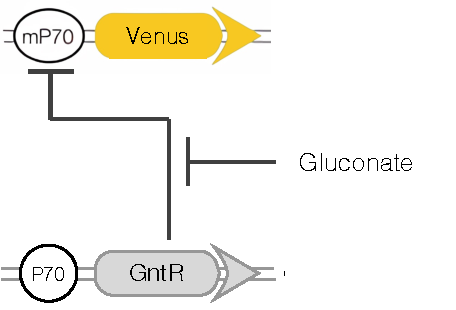
\includegraphics[width=0.45\textwidth]{./figs/fig-0-circuit.pdf}
\end{center}
\caption{Genetic circuit architecture used in this study. The circles represent the promoters for each transcription unit. mP70 is the modified P70 promoter with the GntR operator included. The circuit components were added to the reaction as linear DNA. D-Gluconate was added as a de-repressor at the start of the reaction.}\label{fig:circuit}
\end{figure}

\clearpage

\begin{figure}[h!]
\begin{center}
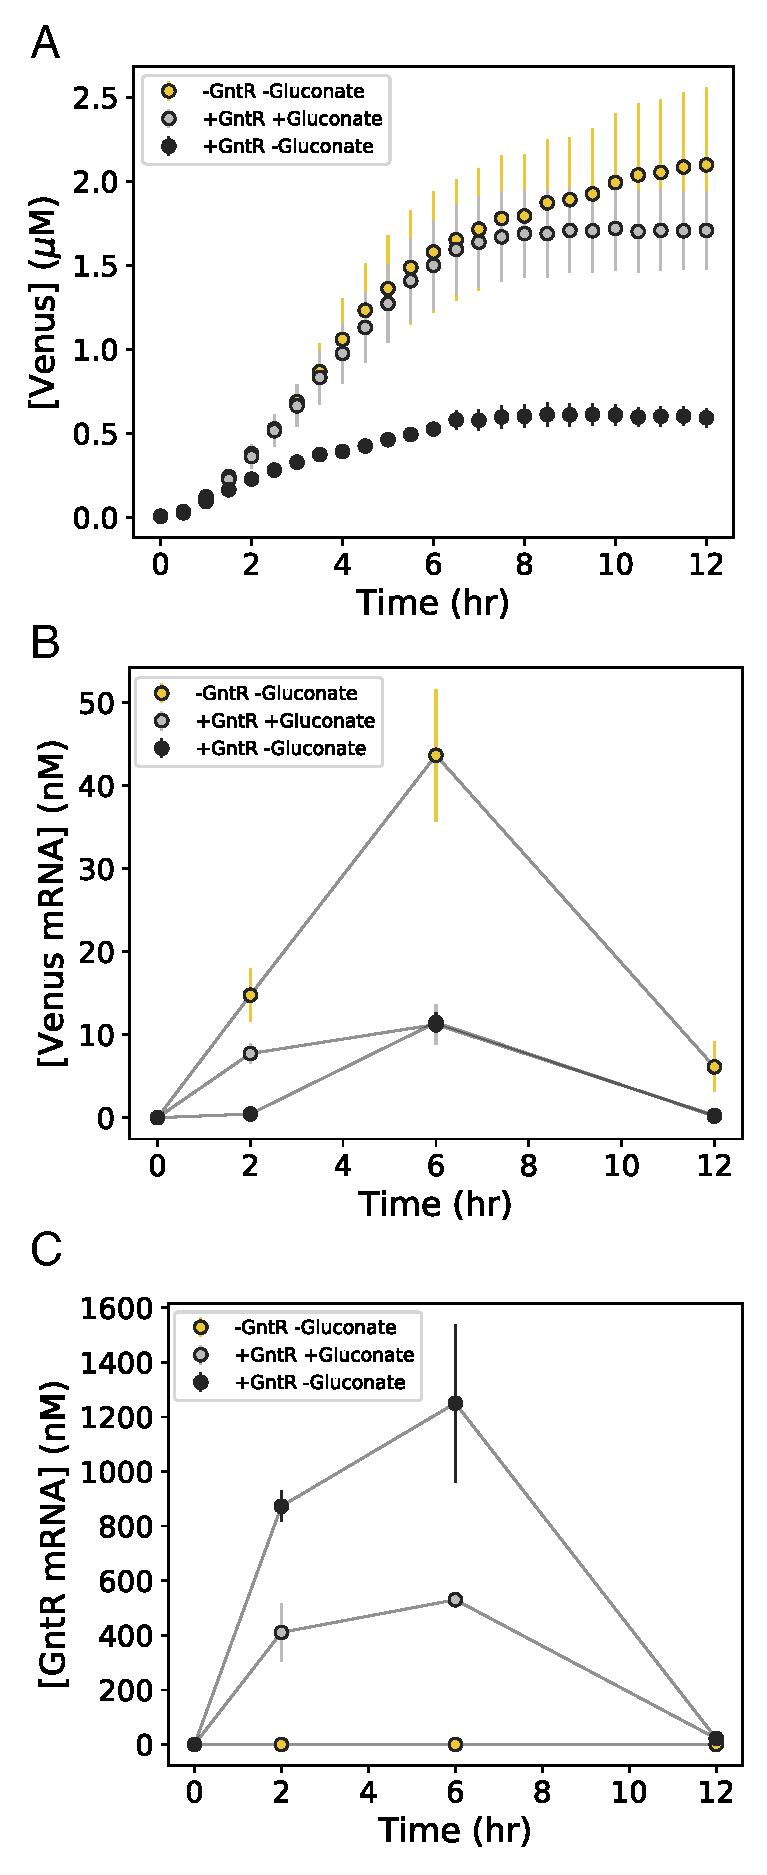
\includegraphics[width=0.45\textwidth]{./figs/fig-1-three-panel.pdf}
\end{center}
\caption{Venus mRNA and protein levels for the three experimental conditions. Linear DNA used were: mP70-Venus (7 nM), P70-GntR (0 or 10 nM).
\textbf{A}: Venus mRNA levels measured using qPCR.
\textbf{B}: Venus protein levels measured on a plate reader (513 nm excitation/531 nm emission).
\textbf{C}: GntR mRNA levels measured using qPCR.
Yellow circles represent the unrepressed case, i.e., without the addition of GntR gene and D-gluconate. Grey circles represent the de-repressed case, i.e., with the addition of both GntR gene (10 nM) and D-gluconate (10 mM). Black circles represent the repressed case, i.e., with only the addition of GntR gene (10 nM). Error bars represent standard errors.}\label{fig:experimental}
\end{figure}

\clearpage

\begin{figure}[h!]
\begin{center}
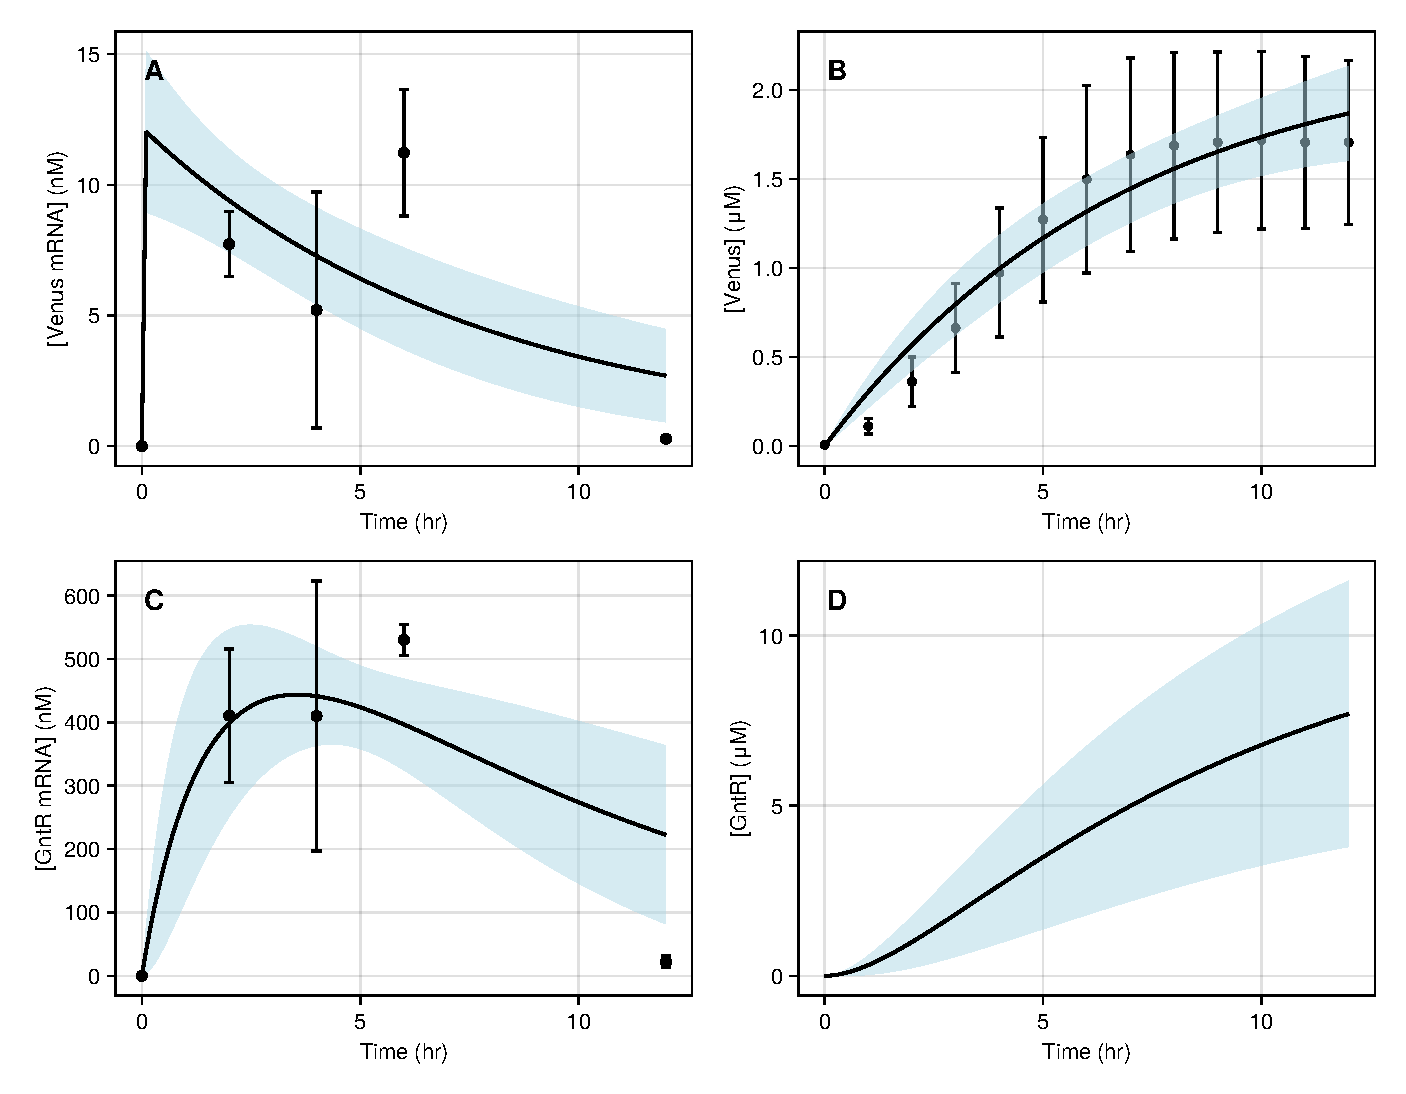
\includegraphics[width=1\textwidth]{./figs/fig_model_training.pdf}
\end{center}
\caption{Mechanistic resource competition model simulations versus experimental measurements for the de-repressed training condition. Linear DNA used were: mP70-Venus (7 nM), P70-GntR (10 nM). D-gluconate (10 mM) was added as the effector at the start of reaction.
\textbf{A}: Venus mRNA.
\textbf{B}: Venus protein (every 12th data point shown for clarity; measurements were collected at 5-minute intervals).
\textbf{C}: GntR mRNA.
\textbf{D}: GntR protein prediction.
Black circles represent experimental data with standard errors captured by error bars across at least three replicates. mRNA was measured using qPCR; Venus protein was measured on a plate reader (513 nm excitation/531 nm emission). The ParetoEnsembles.jl parameter ensemble ($N = 78$) was used to calculate the mean (black line) and 95\% confidence estimate of the model simulation (shaded region). GntR protein (panel D) was predicted by the model and not experimentally measured.}\label{fig:model_training}
\end{figure}

\clearpage

\begin{figure}[h!]
\begin{center}
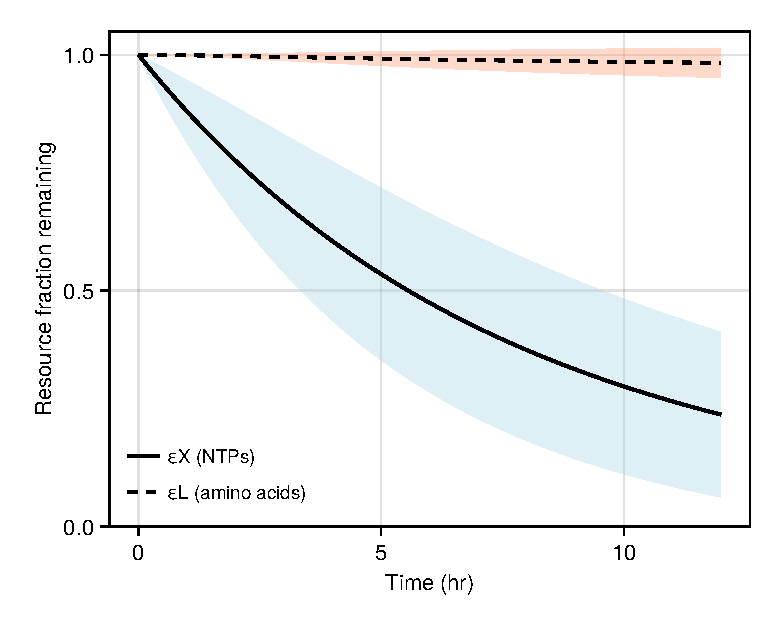
\includegraphics[width=0.6\textwidth]{./figs/fig_resource_depletion.pdf}
\end{center}
\caption{Predicted trajectories of consumable resource availability over the 12-hour cell-free reaction. The transcriptional resource variable $\epsilon_X$ (representing the fractional availability of nucleotides and energy cofactors for transcription) and the translational resource variable $\epsilon_L$ (representing the fractional availability of amino acids and energy cofactors for translation) were computed from the mechanistic resource depletion model (Eqns.~\ref{eq:epsX}--\ref{eq:epsL}). By 12 hours, $\epsilon_X$ declined to 0.24 (76\% depletion) while $\epsilon_L$ declined to 0.98 (2\% depletion), indicating that transcriptional resources were the primary bottleneck. Lines represent the ensemble mean; shaded regions represent the 95\% confidence interval across the parameter ensemble ($N = 78$).}\label{fig:resource_depletion}
\end{figure}

\clearpage

\begin{figure}[h!]
\begin{center}
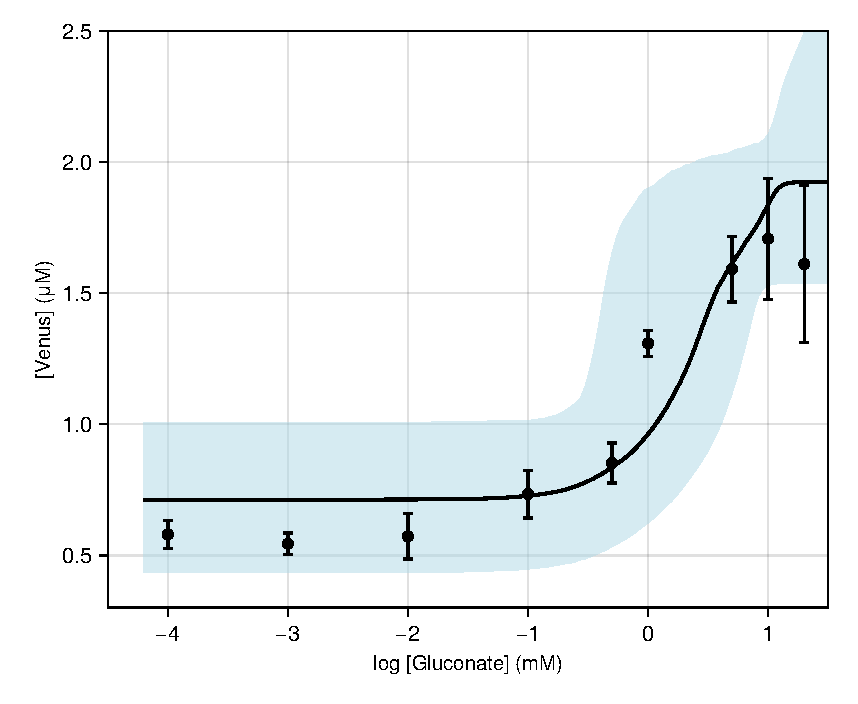
\includegraphics[width=0.6\textwidth]{./figs/fig_dose_response.pdf}
\end{center}
\caption{Model prediction versus experimental measurements for the dose-response study. Linear DNA used were: mP70-Venus (7 nM), P70-GntR (10 nM). D-gluconate concentration was varied from 0.0001 to 20 mM.
Black circles represent Venus protein measurements at the endpoint of the experiment (12 h). Error bars represent standard errors across at least three replicates. The black line represents the ensemble mean of the model prediction, and the shaded region represents the 95\% confidence estimate across the parameter ensemble ($N = 78$). All model parameters were fixed at the values estimated from the 10 mM and 0 mM D-gluconate training conditions; only D-gluconate concentration was varied.}\label{fig:dose_response}
\end{figure}

\clearpage

\begin{table}[ht!]
\centering
\caption{Synthetic fed-batch supplementation analysis. At $t = 3$ hours, the transcriptional ($\epsilon_X$) or translational ($\epsilon_L$) resource fraction was replenished by a supplementation fraction $\phi$. Venus protein concentration at 12 hours (ensemble mean $\pm$ standard deviation, $N = 78$) and fold-change relative to the unsupplemented control are shown. Paired $t$-statistics test the null hypothesis of no difference from the control; all values with $\phi > 0$ were statistically significant ($p < 10^{-10}$), but the $\epsilon_L$ effect was biologically negligible (less than 0.3\%).}
\renewcommand{\arraystretch}{1.1}
\begin{tabular}{ccccccc} \toprule
& \multicolumn{3}{c}{\textbf{TX resource ($\epsilon_X$) boost}} & \multicolumn{3}{c}{\textbf{TL resource ($\epsilon_L$) boost}} \\
\cmidrule(lr){2-4} \cmidrule(lr){5-7}
$\phi$ & Venus ($\mu$M) & Fold-change & $t$-stat & Venus ($\mu$M) & Fold-change & $t$-stat \\ \midrule
0 (control) & $1.87 \pm 0.14$ & 1.00$\times$ & -- & $1.87 \pm 0.14$ & 1.00$\times$ & -- \\
0.25 & $1.71 \pm 0.18$ & 1.13$\times$ & 220 & $1.54 \pm 0.08$ & 1.001$\times$ & 12 \\
0.50 & $1.90 \pm 0.20$ & 1.26$\times$ & 219 & $1.51 \pm 0.17$ & 1.001$\times$ & 12 \\
0.75 & $2.10 \pm 0.23$ & 1.39$\times$ & 217 & $1.51 \pm 0.17$ & 1.002$\times$ & 12 \\
1.00 & $2.29 \pm 0.26$ & 1.52$\times$ & 215 & $1.51 \pm 0.17$ & 1.003$\times$ & 12 \\
\bottomrule
\end{tabular}
\label{table:fedbatch}
\end{table}

\clearpage

\begin{figure}[h!]
\begin{center}
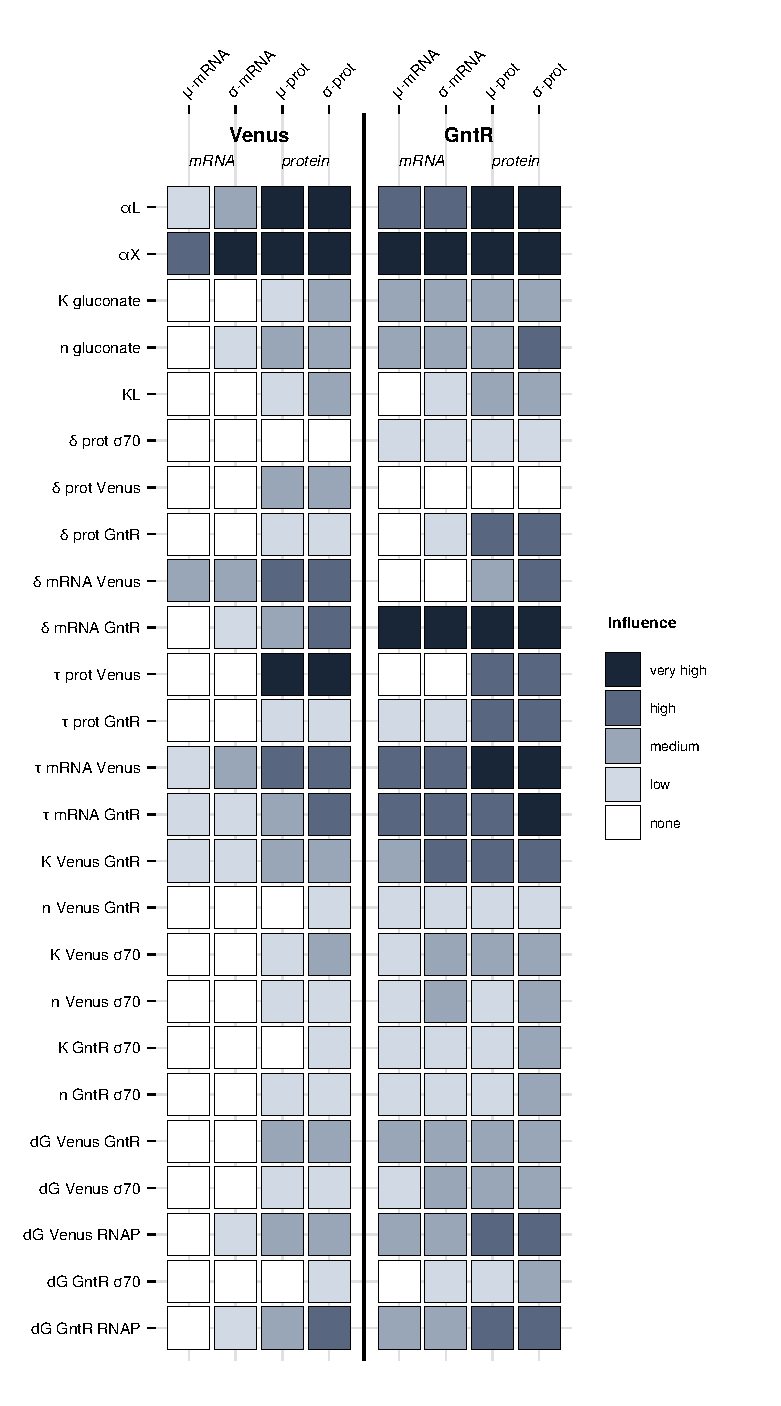
\includegraphics[width=0.8\textwidth]{./figs/fig_sensitivity.pdf}
\end{center}
\caption{Global sensitivity analysis of the model parameters using the Morris method. The heatmap represents the normalized absolute mean elementary effect ($|\mu^{*}|$) of each parameter on four model outputs: Venus mRNA at 6 hours, Venus protein at 12 hours, GntR mRNA at 6 hours, and GntR protein at 12 hours. Values were normalized per output to the range $[0,1]$ for visualization; darker colors indicate greater sensitivity. The resource consumption parameters $\alpha_X$ and $\alpha_L$ were the dominant parameters for all model outputs. Morris sensitivity coefficients were computed over 200 trajectories using parameter ranges derived from the ensemble distribution.}\label{fig:sensitivity}
\end{figure}

\clearpage

\begin{figure}[h!]
\begin{center}
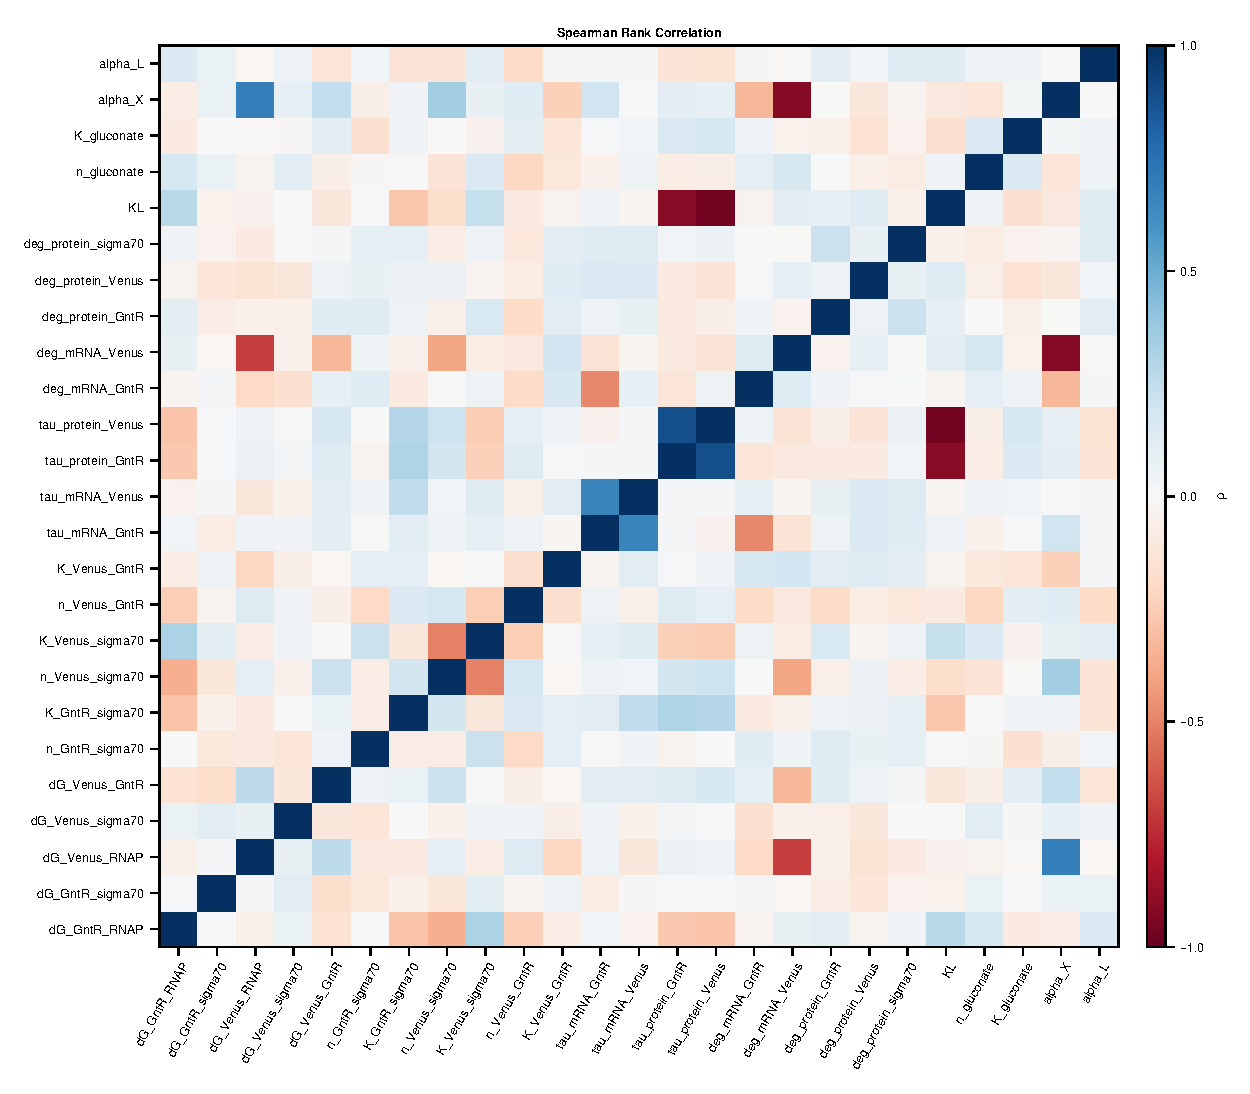
\includegraphics[width=0.8\textwidth]{./figs/fig_correlation_heatmap.pdf}
\end{center}
\caption{Spearman rank correlation matrix of the estimated model parameters across the ensemble ($N = 78$). Strong positive correlations (blue) and negative correlations (red) reveal parameter dependencies that reflect structural identifiability constraints. Notable correlated clusters include the translation time constants ($\tau_{\text{protein,GntR}}$, $\tau_{\text{protein,Venus}}$) and the translation saturation constant ($K_L$), which exhibited pairwise correlations $|\rho| > 0.82$, reflecting the well-known trade-off between Michaelis constant and time constant in enzyme kinetics. The mRNA degradation modifier for GntR was strongly anti-correlated with $\alpha_X$ ($\rho = -0.72$), indicating a compensatory relationship between mRNA stability and transcriptional resource depletion rate.}\label{fig:correlation}
\end{figure}

\clearpage

\begin{table}[ht!]
\centering
\caption{Estimated model parameters for the D-gluconate sensor circuit. Values represent the ensemble mean $\pm$ standard deviation across $N = 78$ parameter sets. The first group contains pseudo-energy parameters for promoter configurations, the second group contains binding and kinetic parameters, and the last two rows are the new resource consumption parameters introduced in this study.}
\renewcommand{\arraystretch}{1.1}
\resizebox{\textwidth}{!}{\begin{tabular}{lcccc} \toprule
\textbf{Description} & \textbf{Parameter} & \textbf{Value} & \textbf{Units} & \textbf{Reference} \\ \toprule
RNA Polymerase concentration & $R_X$ & 0.13 & $\mu$M & set by experiment \\
Ribosome concentration & $R_L$ & 2.0 & $\mu$M & set by experiment \\
Transcription elongation rate & $\dot{v}_X$ & 60 & nt/s & \cite{garamella2016all} \\
Translation elongation rate & $\dot{v}_L$ & 16.5 & aa/s & \cite{garamella2016all} \\
Transcription saturation coeff. & $K_X$ & 0.054 & $\mu$M & \cite{mcclure_1980} \\
Transcription initiation time & $k_{\text{init},X}$ & 22 & s & \cite{mcclure_1980} \\
Translation initiation time & $k_{\text{init},L}$ & 1.5 & s & \cite{adhikari2020effective} \\
Venus gene length & $l_{G,\text{Venus}}$ & 720 & nt & from DNA sequence \\
GntR gene length & $l_{G,\text{GntR}}$ & 996 & nt & from DNA sequence \\
& & & & \\
cRNAP + P70 pseudo-energy & $\epsilon_{P70,cRNAP}$ & $0.082 \pm 0.20$ & $k_BT$ & -- \\
hRNAP + P70 pseudo-energy & $\epsilon_{P70,hRNAP}$ & $-0.21 \pm 0.35$ & $k_BT$ & -- \\
cRNAP + mP70 pseudo-energy & $\epsilon_{mP70,cRNAP}$ & $0.40 \pm 0.38$ & $k_BT$ & -- \\
hRNAP + mP70 pseudo-energy & $\epsilon_{mP70,hRNAP}$ & $-0.11 \pm 0.18$ & $k_BT$ & -- \\
GntR + mP70 operator & $\epsilon_{mP70,GntR}$ & $-1.64 \pm 0.45$ & $k_BT$ & -- \\
& & & & \\
Hill coeff. P70 + hRNAP & $n_{P70,hRNAP}$ & $2.01 \pm 2.29$ & -- & -- \\
Dissoc. const. P70 + hRNAP & $K_{P70,hRNAP}$ & $0.046 \pm 0.065$ & $\mu$M & -- \\
Hill coeff. mP70 + hRNAP & $n_{mP70,hRNAP}$ & $1.61 \pm 1.51$ & -- & -- \\
Dissoc. const. mP70 + hRNAP & $K_{mP70,hRNAP}$ & $22.1 \pm 26.2$ & $\mu$M & -- \\
Hill coeff. mP70 + GntR & $n_{mP70,GntR}$ & $5.39 \pm 3.10$ & -- & -- \\
Dissoc. const. mP70 + GntR & $K_{mP70,GntR}$ & $0.0032 \pm 0.0041$ & $\mu$M & -- \\
& & & & \\
TX time const. GntR & $\tau_{X,GntR}$ & $2.14 \pm 1.98$ & -- & -- \\
TX time const. Venus & $\tau_{X,Venus}$ & $0.076 \pm 0.085$ & -- & -- \\
TL time const. GntR & $\tau_{L,GntR}$ & $6.53 \pm 4.77$ & -- & -- \\
TL time const. Venus & $\tau_{L,Venus}$ & $0.48 \pm 0.37$ & -- & -- \\
Deg. modifier mRNA GntR & $\delta_{m,GntR}$ & $0.029 \pm 0.017$ & -- & -- \\
Deg. modifier mRNA Venus & $\delta_{m,Venus}$ & $41.8 \pm 28.0$ & -- & -- \\
Deg. modifier protein GntR & $\delta_{p,GntR}$ & $0.012 \pm 0.024$ & -- & -- \\
Deg. modifier protein Venus & $\delta_{p,Venus}$ & $0.20 \pm 0.25$ & -- & -- \\
Deg. modifier protein $\sigma_{70}$ & $\delta_{p,\sigma_{70}}$ & $0.0019 \pm 0.0020$ & -- & -- \\
Translation saturation const. & $K_L$ & $569 \pm 277$ & $\mu$M & -- \\
& & & & \\
Hill coeff. gluconate-GntR & $n_{\text{gluconate}}$ & $2.36 \pm 0.34$ & -- & -- \\
Dissoc. const. gluconate-GntR & $K_{\text{gluconate}}$ & $0.13 \pm 0.01$ & mM & -- \\
& & & & \\
TX resource consumption rate & $\alpha_X$ & $(2.2 \pm 1.2) \times 10^{-5}$ & $(\mu\text{M}\cdot\text{nt}\cdot\text{hr})^{-1}$ & -- \\
TL resource consumption rate & $\alpha_L$ & $(5.6 \pm 5.0) \times 10^{-6}$ & $(\mu\text{M}\cdot\text{aa}\cdot\text{hr})^{-1}$ & -- \\
\bottomrule
\end{tabular}}
\label{table:model-parameters}
\end{table}

\clearpage

% Supplemental information
\renewcommand\thefigure{S\arabic{figure}}
\renewcommand\thetable{T\arabic{table}}
\renewcommand\thepage{S-\arabic{page}}
\renewcommand\theequation{S\arabic{equation}}

\setcounter{equation}{0}
\setcounter{table}{0}
\setcounter{figure}{0}

\section*{Supplemental Information}

\begin{figure}[h!]
\begin{center}
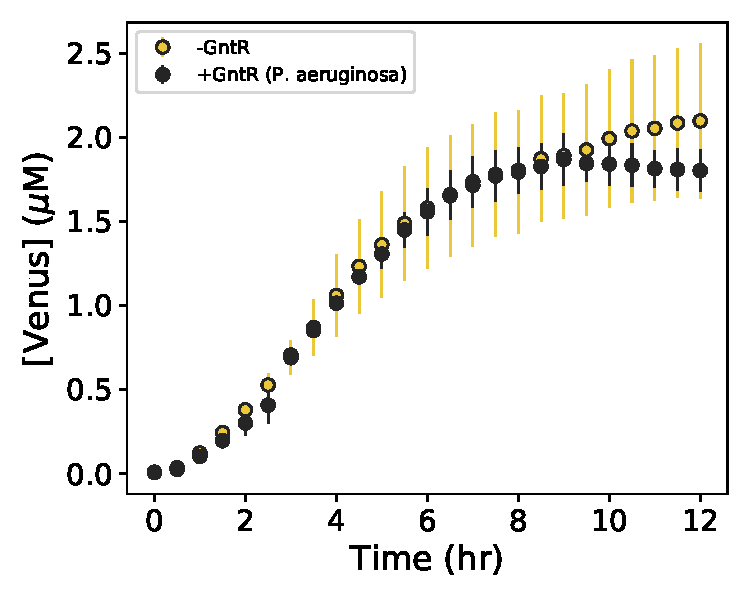
\includegraphics[width=0.6\textwidth]{./figs/fig-S1-resource_limitation_Pseudomonas.pdf}
\end{center}
\caption{Venus protein levels measured for two cases: addition of \textit{P.~aeruginosa} GntR gene and in the absence of GntR gene. Linear DNA used were: mP70-Venus (7 nM), P70-GntR (0 or 10 nM). The \textit{P.~aeruginosa} GntR variant does not bind to the \textit{E.~coli} GntR operator, serving as a control for resource competition effects.}\label{fig:S1}
\end{figure}

\end{document}
